\section{Structure du frontend}
Pour commencer ce chapitre, je pense qu'il est important de préciser la structure de cette partie du projet. Le code se trouve dans le dossier \emph{src} du projet.
Il est organisé de la manière suivante :
\begin{itemize}
    \item \emph{assets} : Contient toutes les images utilisée dans le projet.
    \item \emph{components} : Contient tous les composants qui seront utilisés dans les vues.
    \item \emph{middleware} : Contient le middleware permettant de vérifier si l'utilisateur est connecté ou non et quels sont ses droits.
    \item \emph{router} : Contient la liste de toutes les routes de l'application
    \item \emph{stores} : Contient les fichiers permettant de gérer les données du \emph{frontend} et le code permettant de faire des requêtes à l'API.
    \item \emph{views} : Contient les différentes vues de l'application.
\end{itemize}

Cette structure organisée permet de faciliter la maintenance et la reprise du projet en répartissant les différents éléments dans les dossiers appropriés.

\section{Communication avec le backend}
La communication entre le \emph{frontend} et le \emph{backend} s'effectue à l'aide de requêtes \emph{fetch}. Étant donné que de nombreux composants du \emph{frontend} ont besoin de communiquer avec le \emph{backend}, un fichier \emph{utils.js} a été dans le dossier \emph{src} contenant une fonction permettant de faire des requêtes \emph{fetch} à l'API. Cette approche de centralisation permet de factoriser le code et de faciliter d'éventuelles modifications ultérieures.


\begin{listing}[H]
    \inputminted{js}{assets/code/communcation.vue}
    \caption{Communication avec le backend}
\end{listing}

Cette fonction prend en paramètre une \emph{url}, et un objet contenant les paramètres de la requête. Son objectif est de fournir une approche unifiée pour différentes requêtes HTTP telles que \emph{GET, POST, PATCH, PUT} et \emph{DELETE}. Il est également possible de rajouter des données au format \emph{JSON} dans le corps de la requête. On y voit également deux constantes qui sont définies dans le fichier \emph{.env} du projet. Cela permet de changer l'adresse du backend sans avoir à changer le code.

Pour mieux illustrer son utilisation, un exemple concret sera présenté dans la section \emph{Store} ci-dessous.

\section{Store}
Les stores jouent un rôle essentiel dans cette partie du projet. Ils permettent de stocker des données directement dans le \emph{frontend} de l'application, évitant ainsi des requêtes trop fréquente à l'API qui auraient un impact négatif sur les performances de l'application. De plus, les stores permettent de centraliser les différents appels à l'API, ce qui contribue à une meilleure organisation et factorisation du code.

Un exemple très parlant de leur utilité est la gestion des informations d'un utilisateur connecté. S'il était nécessaire de faire un appel supplémentaire à l'API à chaque changement de vue ou de composant, cela serait coûteux en performance.
Voici un extrait de code du \emph{store user} :

\begin{listing}[H]
    \inputminted{js}{assets/code/userStore.js}
    \caption{Store utilisateur}
\end{listing}

On peut voir l'import du fichier \emph{utils.js} ainsi que l'utilisation de la fonction \emph{fetchApi}.
L'objet \emph{user} est déclaré pour stocker les informations de l'utilisateur connecté.

Un point intéressant est que la fonction \emph{fetchUser} vérifie si l'objet \emph{user} est vide avant de faire un appel à l'API. Si les informations sont déjà en possession, un appel à l'API est donc évité. Lors de l'utilisation de cette fonction dans les composants et vues, on n'a pas à se soucier de savoir si l'appel est redondant. Cela permet de grandement simplifier le code.

La fonction \emph{logout} permet de déconnecter l'utilisateur. Cette fonction ne fait que supprimer l'objet \emph{user} du \emph{store}, car c'est l'API qui gère la connexion ainsi que la déconnexion.

Finalement, en bas du fichier, on peut voir un \emph{return} qui expose les fonctions et variables du \emph{store} aux composants et vues.

Tous les \emph{stores} de ce projet suivent une structure similaire à celle-ci.

\section{Middleware}
L'un des gros défauts de l'ancien \emph{fontend} est qu'il n'y avait aucune logique empêchant un utilisateur non connecté d'accéder à des pages nécessitant une connexion. Cette lacune pouvait entraîner toutes sortes de bugs et d'incohérences dans le fonctionnement de l'application. De plus, l'utilisateur non connecté ou ne disposant pas des droits nécessaires ne pouvait pas utiliser ces pages correctement. Ce qui constitue donc un problème autant d'un point de vue sécurité que de l'expérience utilisateur. Il est donc impératif de le régler.

Pour palier à cela, deux \emph{middleware} ont été mis en place en se basant sur cet article \cite{middlewareVuejs}.

Dans un premier temps, il faut créer un fichier \emph{auth.js} dans le dossier \emph{middleware} du projet. Il y a également un \emph{middleware} pour les enseignants qui a été créé mais son code, très similaire à celui-ci, ne sera pas montré.

\begin{listing}[H]
    \inputminted{js}{assets/code/auth.js}
    \caption{Middleware authentication}
\end{listing}
Ce code présente une fonction qui utilise le \emph{store} pour vérifier si l'utilisateur est connecté. Si ce n'est pas le cas, on le redirige vers la vue \emph{root}, sinon on le laisse accéder à la page demandée.

Ensuite, un autre fichier nommé \emph{middleware-pipeline.js} est créé dans le même dossier.
\begin{listing}[H]
    \inputminted{js}{assets/code/middlewarePipeline.js}
    \caption{Middleware pipeline}
\end{listing}

Cette fonction prend un tableau de \emph{middleware} en paramètre et traverse ce tableau en appliquant chacun des \emph{middleware}. Si l'un des \emph{middleware} bloque l'accès à l'utilisateur, le processus se termine et l'utilisateur est redirigé vers la page \emph{root}. Si tous les \emph{middleware} autorisent l'accès, alors l'utilisateur est autorisé à atteindre cette ressource.


Finalement, dans le fichier \emph{index.js} du dossier \emph{router}, on ajoute ce code :

\begin{listing}[H]
    \inputminted{js}{assets/code/beforeEachRoute.js}
    \caption{Actions effecutées avant chaque route}
\end{listing}

Ceci permet de définir une action qui sera exécutée avant chaque accès à une route.

On peut ajouter un certain \emph{middleware} à la déclaration d'une route de la manière :

\begin{listing}[H]
    \inputminted{js}{assets/code/route.js}
    \caption{Utilisation du middleware}
\end{listing}


\section{Changements graphiques}
Suite à la refonte du \emph{frontend} avec TailwindCSS, de nombreux changements ont été apportés. Bien que l'interface ait été modifiée, beaucoup de pages sont restées relativement similaires. Seuls les changements les plus importants seront présentés ici.

\subsection{Popup d'information}
Un problème majeur de l'ancien \emph{frontend} était l'absence de \emph{popup} d'information informant l'utilisateur du succès ou de l'échec d'une action. Parfois, même si tout fonctionnait comme prévu, en l'absence d'information visuelle, l'utilisateur pouvait penser que l'action n'avait pas été effectuée.
C'est pourquoi une popup d'information a été ajoutée. Il permet d'afficher un message à l'utilisateur et est utilisé dans la plupart les composants et vues du projet.

Voici un exemple d'utilisation de cette \emph{popup} :
\begin{center}
    \begin{figure}[H]
        
\includegraphics[width=\textwidth]{./assets/figures/validationPopup.png}
        \caption{Popup d'information}
    \end{figure}
\end{center}

Une variante de cette même \emph{popup} est utilisée pour signaler les erreurs :
\begin{center}
    \begin{figure}[H]
        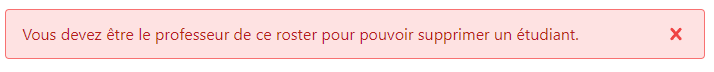
\includegraphics[width=\textwidth]{./assets/figures/errorPopup.png}
        \caption{Popup d'erreur}
    \end{figure}
\end{center}

\subsection{Menu}
Le menu de l'ancienne application n'étant pas très intuitif et ne s'adaptait pas à au rôle de l'utilisateur. Il s'adapte désormais au rôle de ce dernier et comporte des menu déroulant.

\begin{center}
    \begin{figure}[H]
        
\includegraphics[width=\textwidth]{./assets/figures/basicNav.png}
        \caption{Menu utilisateur non connecté}
    \end{figure}
\end{center}

\begin{center}
    \begin{figure}[H]
        
\includegraphics[width=\textwidth]{./assets/figures/teacherNav.png}
        \caption{Menu enseignant}
    \end{figure}
\end{center}

\begin{center}
    \begin{figure}[H]
        
\includegraphics[width=\textwidth]{./assets/figures/studentNav.png}
        \caption{Menu élève}
    \end{figure}
\end{center}

\subsection{Documentation}
Afin de faciliter la compréhension de la création de quiz et de questions, une page supplémentaire dédiée à la documentation a été ajoutée.

\begin{center}
    \begin{figure}[H]
        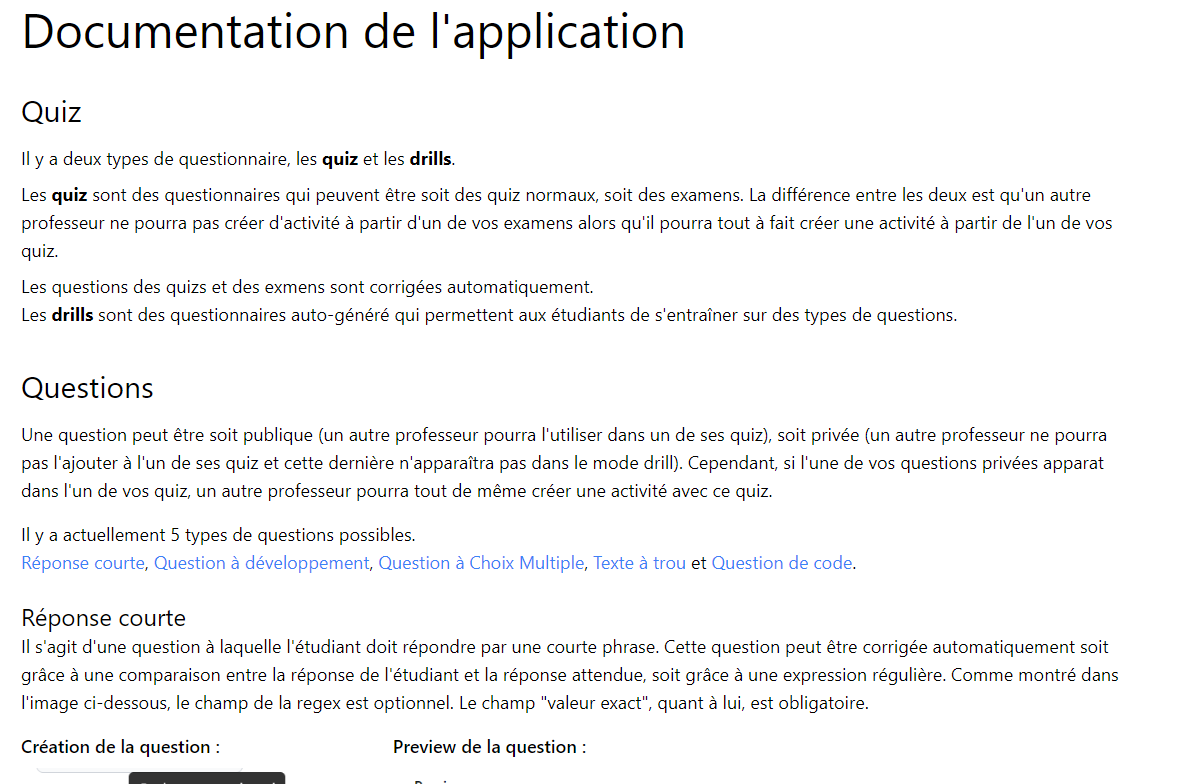
\includegraphics[width=\textwidth]{./assets/figures/documentation.png}
        \caption{Page de documentation de l'application}
    \end{figure}
\end{center}

\subsection{Page 404}
Une page par défaut a été mise en place lorsque l'utilisateur entre une \emph{URL} qui ne correspond à aucune vue existante.

\begin{center}
    \begin{figure}[H]
        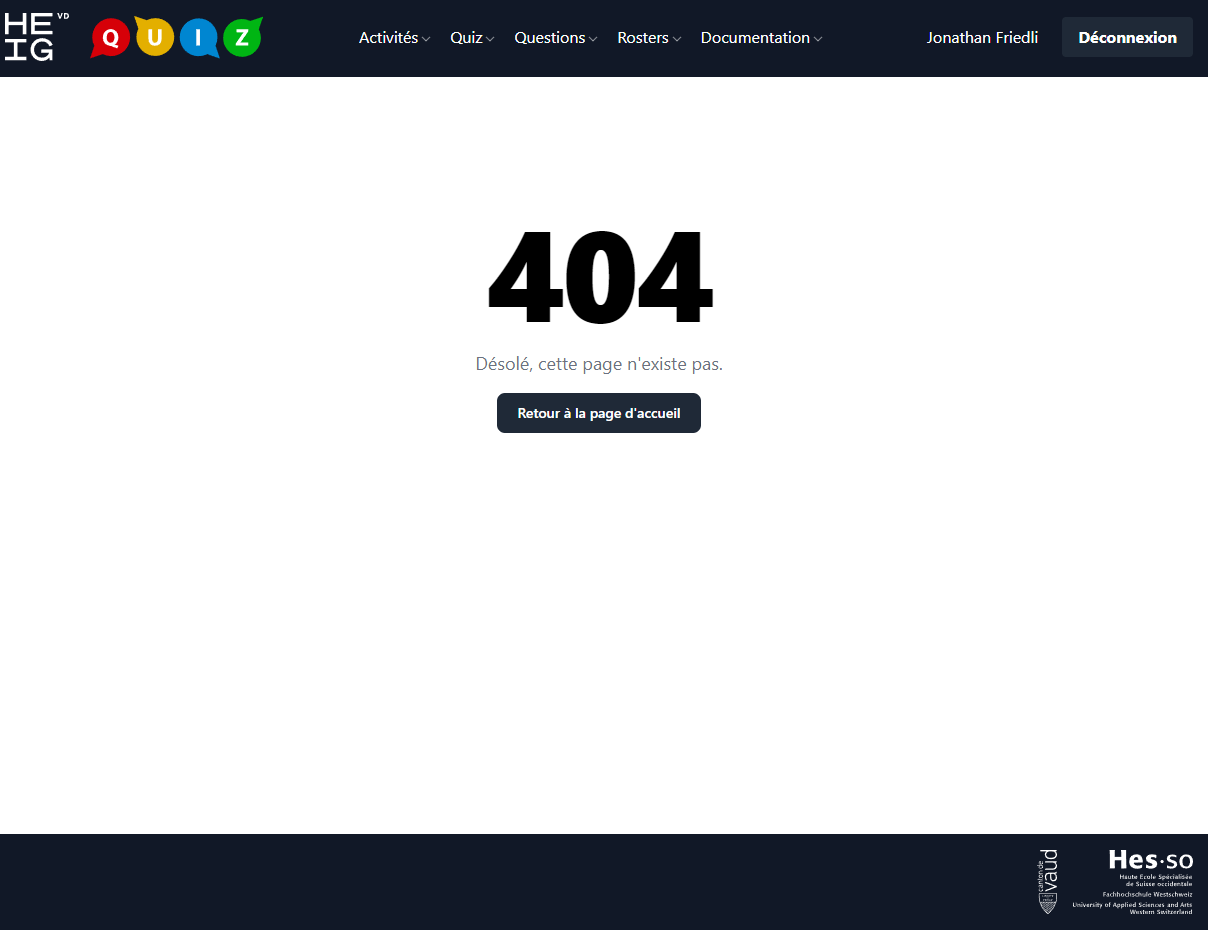
\includegraphics[width=\textwidth]{./assets/figures/page404.png}
        \caption{Page non trouvée}
    \end{figure}
\end{center}


\section{Compilation de code}
La fonctionnalité permettant de compiler le code a été réalisée dans un composant réutilisable. Ce qui permet d'utiliser cette dernière à la fois dans la \emph{preview} lors de la création ou modification, mais également lors d'un quiz, d'un examen ou d'un \emph{drill}.
Voici à un aperçu du fonctionnement :
\begin{center}
    \begin{figure}[H]
        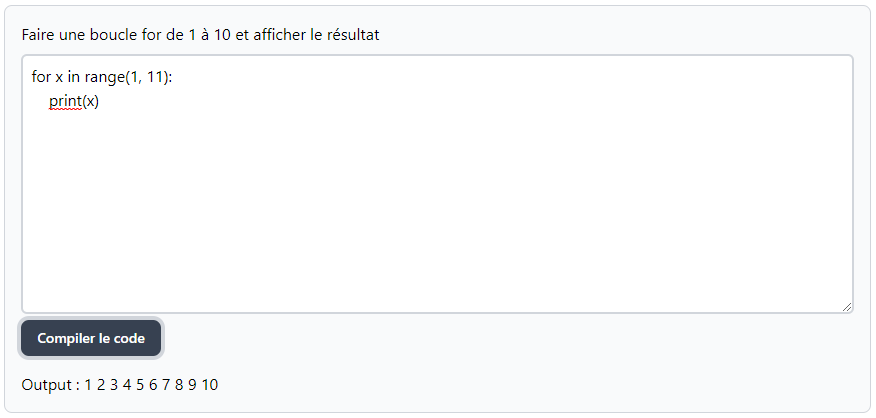
\includegraphics[width=\textwidth]{./assets/figures/codeCompilation.png}
        \caption{Compilation de code}
    \end{figure}
\end{center}

En cas d'erreur dans le code saisi, le comportement est également géré de manière appropriée :
\begin{center}
    \begin{figure}[H]
        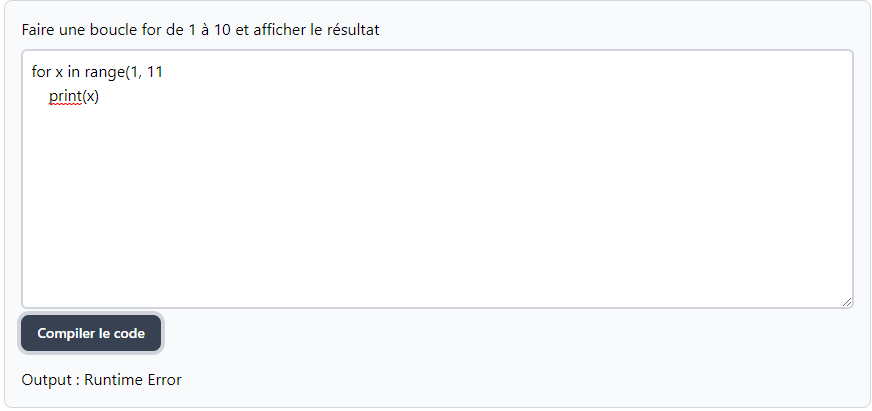
\includegraphics[width=\textwidth]{./assets/figures/codeCompilationError.png}
        \caption{Compilation de code avec erreur}
    \end{figure}
\end{center}

\section{Quiz et examens}
Les quiz et les examens sont entièrement fonctionnels. Ils partagent tous deux le même composant. La différence est que si un étudiant rend un examen en avance, il ne pourra plus y accéder. Tandis que si ce dernier rend un quiz en avance, il peut toujours revenir et modifier ses réponses. Cette mesure a été mise en place pour prévenir toute tentative de triche.

De plus, un détail important à noter est que les questions se chargent au fur et à mesure. Lorsqu'un étudiant accède à une question pour la première fois, l'application fait une requête à l'API afin de récupérer les informations. Ensuite, ces dernières sont stockées dans le \emph{store} de l'activité afin de rendre l'application la plus fluide possible.

Exemple de quiz :

\begin{center}
    \begin{figure}[H]
        
\includegraphics[width=\textwidth]{./assets/figures/quizExample.png}
        \caption{Exemple de quiz}
    \end{figure}
\end{center}

\section{Drill}
Le mode \emph{drill} se décompose en deux parties. Tout d'abord, l'utilisateur sélectionne un mot-clé parmi les choix proposés.


\begin{center}
    \begin{figure}[H]
        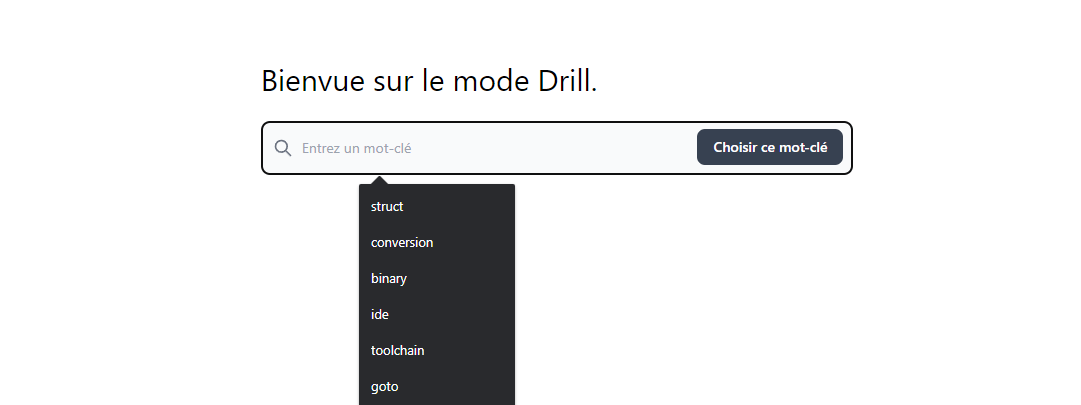
\includegraphics[width=\textwidth]{./assets/figures/drill1.png}
        \caption{Choix du mot-clé}
    \end{figure}
\end{center}

Une fois cette étape effectuée, l'utilisateur est redirigé sur une nouvelle page contenant uniquement des questions publiques associées au mot-clé choisi.
Un chronomètre démarre alors et l'utilisateur doit répondre à la question.
\begin{center}
    \begin{figure}[H]
        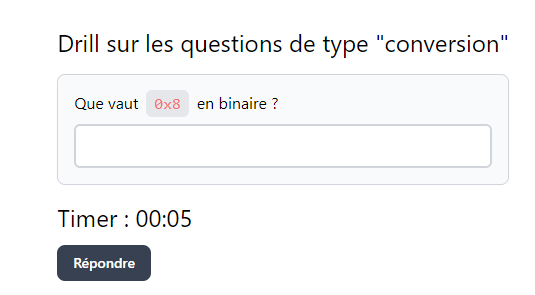
\includegraphics[width=\textwidth]{./assets/figures/drill2.png}
        \caption{Question en mode drill}
    \end{figure}
\end{center}

Une fois sa réponse validée, l'utilisateur peut voir la bonne réponse et l'application indique si sa réponse a été acceptée ou non.

\begin{center}
    \begin{figure}[H]
        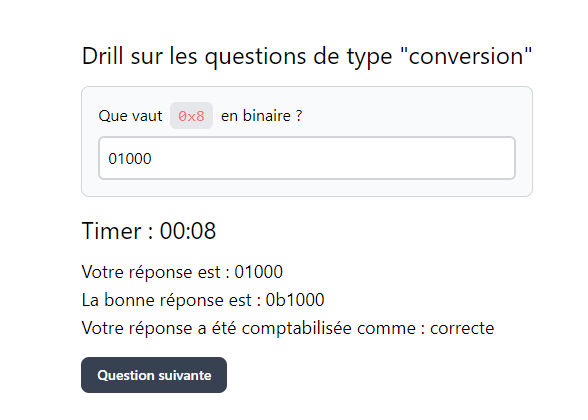
\includegraphics[width=\textwidth]{./assets/figures/drill3.png}
        \caption{Réponse du mode drill}
    \end{figure}
\end{center}

En fonction de sa réponse, cette question reviendra plus ou moins vite. L'utilisateur peut alors cliquer sur le bouton "question suivante" pour continuer le \emph{drill}.
Une fois que l'utilisateur a répondu à toutes les questions, il n'est pas obligé d'attendre le jour suivant pour continuer de répondre aux questions. Ce choix a été fait afin d'éviter que l'utilisateur ait à attendre un où plusieurs jours pour ne répondre qu'a une ou deux questions. Ce qui pourrait être le cas si seulement une dizaine question sont affiliés à certains mots-clés spécifiques.